% Full flowchart of the formulation-4 RL (2026-11-22_formulation_4/baseline_RL/code):
% training (train_rl_f4.py), one episode (rl_f4_model.rollout + rl_f4_env.Env) and inference (solve_rl_f4.py).
% Compile: pdflatex flowchart.tex
\documentclass[border=6pt]{standalone}
\usepackage{lmodern}
\usepackage[T1]{fontenc}
\usepackage{amsmath,amssymb}
\usepackage{tikz}
\usetikzlibrary{arrows.meta,shapes.geometric,shapes.misc,fit,backgrounds,calc}
\begin{document}
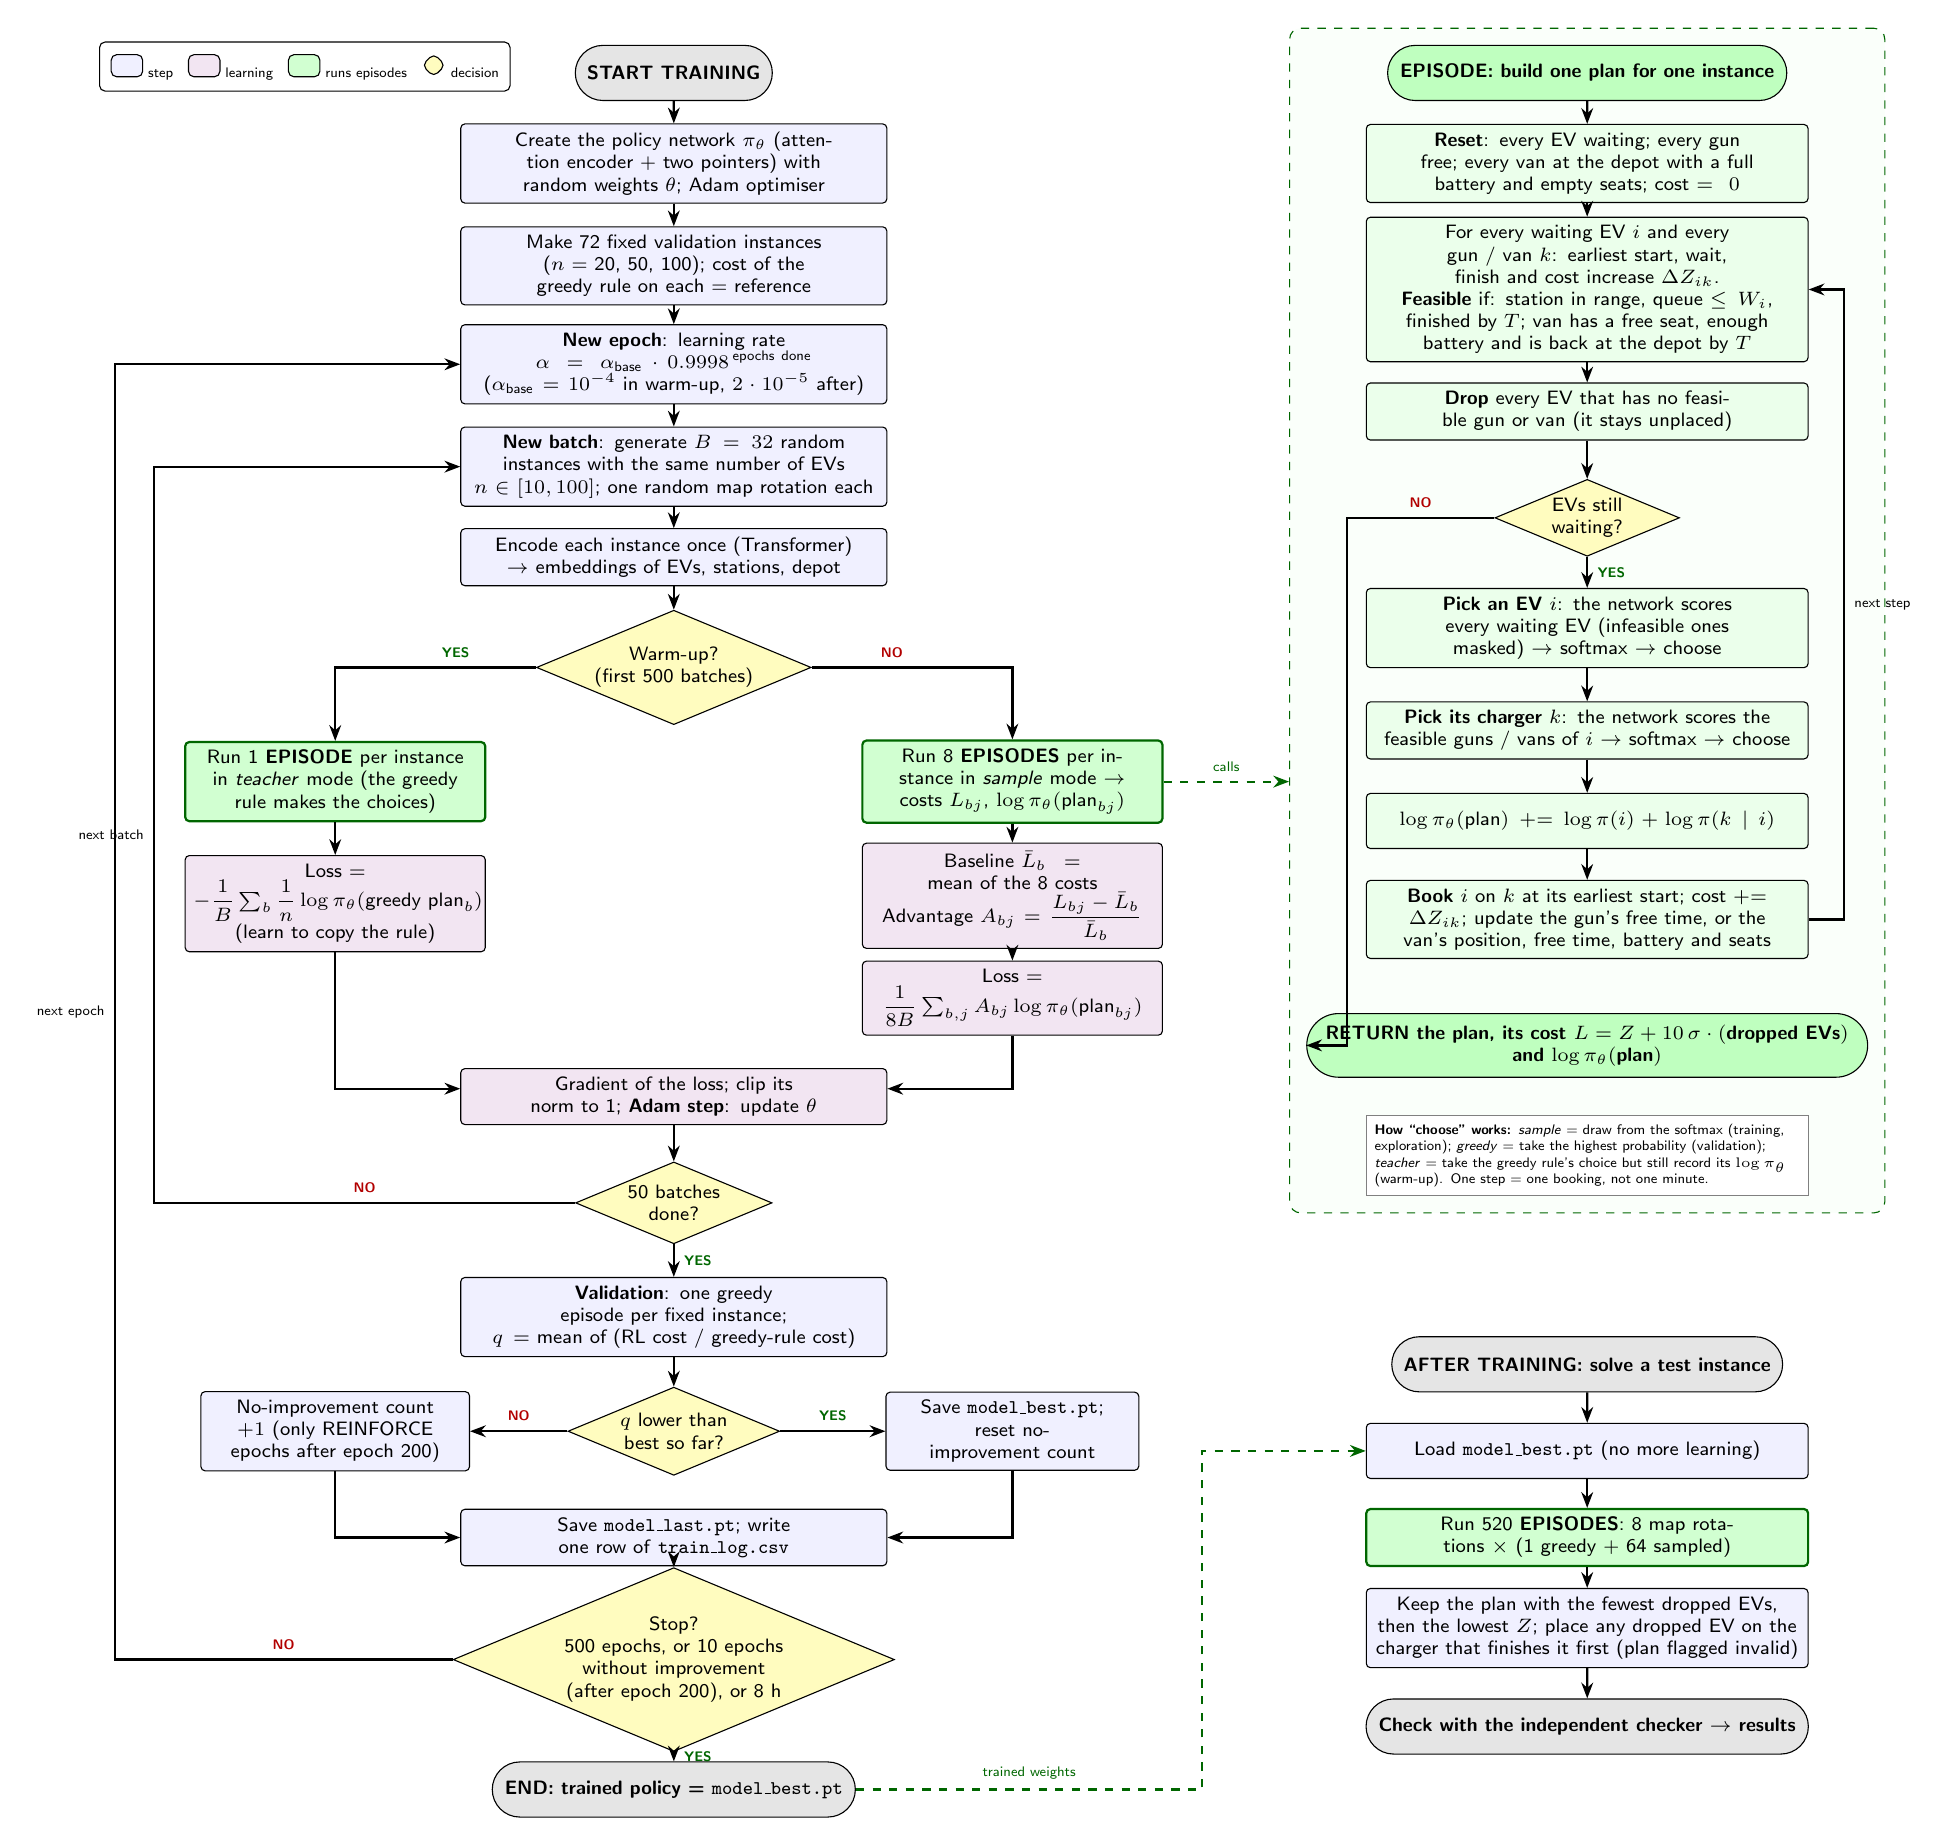
\begin{tikzpicture}[
  font=\sffamily\scriptsize, >={Stealth[length=2mm]},
  term/.style={rounded rectangle, draw, fill=gray!20, align=center, inner sep=4pt, minimum height=7mm, font=\sffamily\scriptsize\bfseries},
  proc/.style={rectangle, rounded corners=1.5pt, draw, fill=blue!6, align=center, text width=#1, inner sep=3pt, minimum height=7mm},
  proc/.default=5.2cm,
  learn/.style={proc=#1, fill=violet!10},
  learn/.default=5.2cm,
  epi/.style={proc=#1, fill=green!8},
  epi/.default=5.4cm,
  dec/.style={diamond, draw, fill=yellow!25, aspect=2.4, align=center, inner sep=1pt, font=\sffamily\scriptsize},
  call/.style={proc=#1, fill=green!18, draw=green!40!black, thick},
  call/.default=3.6cm,
  arr/.style={->, thick},
  yes/.style={font=\sffamily\tiny\bfseries, text=green!40!black},
  no/.style={font=\sffamily\tiny\bfseries, text=red!70!black},
  dashcall/.style={->, thick, dashed, green!40!black},
]
% ================================================================== TRAINING (left)
\node[term] (start) at (0,0) {START TRAINING};
\node[proc] (init) at (0,-1.15) {Create the policy network $\pi_\theta$ (attention encoder + two pointers) with random weights $\theta$; Adam optimiser};
\node[proc] (val0) at (0,-2.45) {Make 72 fixed validation instances ($n$ = 20, 50, 100); cost of the greedy rule on each = reference};
\node[proc] (ep) at (0,-3.7) {\textbf{New epoch}: learning rate $\alpha=\alpha_{\text{base}}\cdot 0.9998^{\,\text{epochs done}}$\\ ($\alpha_{\text{base}}=10^{-4}$ in warm-up, $2\cdot10^{-5}$ after)};
\node[proc] (gen) at (0,-5.0) {\textbf{New batch}: generate $B=32$ random instances with the same number of EVs $n\in[10,100]$; one random map rotation each};
\node[proc] (enc) at (0,-6.15) {Encode each instance once (Transformer) $\to$ embeddings of EVs, stations, depot};
\node[dec] (warm) at (0,-7.55) {Warm-up?\\(first 500 batches)};

% warm-up branch (left)
\node[call] (wcall) at (-4.3,-9.0) {Run 1 \textbf{EPISODE} per instance in \emph{teacher} mode (the greedy rule makes the choices)};
\node[learn=3.6cm] (wloss) at (-4.3,-10.55) {Loss $=-\dfrac1B\sum_b\dfrac1n\log\pi_\theta(\text{greedy plan}_b)$\\ (learn to copy the rule)};
% REINFORCE branch (right)
\node[call] (rcall) at (4.3,-9.0) {Run 8 \textbf{EPISODES} per instance in \emph{sample} mode $\to$ costs $L_{bj}$, $\log\pi_\theta(\text{plan}_{bj})$};
\node[learn=3.6cm] (adv) at (4.3,-10.45) {Baseline $\bar L_b=$ mean of the 8 costs\\ Advantage $A_{bj}=\dfrac{L_{bj}-\bar L_b}{\bar L_b}$};
\node[learn=3.6cm] (rloss) at (4.3,-11.75) {Loss $=\dfrac{1}{8B}\sum_{b,j}A_{bj}\log\pi_\theta(\text{plan}_{bj})$};

\node[learn] (adam) at (0,-13.0) {Gradient of the loss; clip its norm to 1; \textbf{Adam step}: update $\theta$};
\node[dec] (bat) at (0,-14.35) {50 batches\\done?};
\node[proc] (val) at (0,-15.8) {\textbf{Validation}: one greedy episode per fixed instance;\\ $q=$ mean of (RL cost / greedy-rule cost)};
\node[dec] (better) at (0,-17.25) {$q$ lower than\\ best so far?};
\node[proc=3.0cm] (best) at (4.3,-17.25) {Save \texttt{model\_best.pt};\\ reset no-improvement count};
\node[proc=3.2cm] (stale) at (-4.3,-17.25) {No-improvement count $+1$ (only REINFORCE epochs after epoch 200)};
\node[proc] (save) at (0,-18.6) {Save \texttt{model\_last.pt}; write one row of \texttt{train\_log.csv}};
\node[dec] (stop) at (0,-20.15) {Stop?\\ 500 epochs, or 10 epochs\\ without improvement\\ (after epoch 200), or 8 h};
\node[term] (end) at (0,-21.8) {END: trained policy = \texttt{model\_best.pt}};

% training arrows
\draw[arr] (start) -- (init);
\draw[arr] (init) -- (val0);
\draw[arr] (val0) -- (ep);
\draw[arr] (ep) -- (gen);
\draw[arr] (gen) -- (enc);
\draw[arr] (enc) -- (warm);
\draw[arr] (warm.west) -| node[yes, above, pos=0.2]{YES} (wcall.north);
\draw[arr] (warm.east) -| node[no, above, pos=0.2]{NO} (rcall.north);
\draw[arr] (wcall) -- (wloss);
\draw[arr] (rcall) -- (adv);
\draw[arr] (adv) -- (rloss);
\draw[arr] (wloss.south) |- ($(adam.west)+(0,0.1)$);
\draw[arr] (rloss.south) |- ($(adam.east)+(0,0.1)$);
\draw[arr] (adam) -- (bat);
\draw[arr] (bat.west) -- node[no, above]{NO} (-6.6,-14.35) |- node[pos=0.25, left, font=\sffamily\tiny]{next batch} (gen.west);
\draw[arr] (bat) -- node[yes, right]{YES} (val);
\draw[arr] (val) -- (better);
\draw[arr] (better.east) -- node[yes, above]{YES} (best);
\draw[arr] (better.west) -- node[no, above]{NO} (stale);
\draw[arr] (best.south) |- ($(save.east)+(0,0)$);
\draw[arr] (stale.south) |- ($(save.west)+(0,0)$);
\draw[arr] (save) -- (stop);
\draw[arr] (stop.west) -- node[no, above]{NO} (-7.1,-20.15) |- node[pos=0.25, left, font=\sffamily\tiny]{next epoch} (ep.west);
\draw[arr] (stop) -- node[yes, right]{YES} (end);

% ================================================================== EPISODE (right)
\begin{scope}[xshift=11.6cm]
\node[term, fill=green!25] (e0) at (0,0) {EPISODE: build one plan for one instance};
\node[epi] (reset) at (0,-1.15) {\textbf{Reset}: every EV waiting; every gun free; every van at the depot with a full battery and empty seats; cost $=0$};
\node[epi] (opt) at (0,-2.75) {For every waiting EV $i$ and every gun / van $k$: earliest start, wait, finish and cost increase $\Delta Z_{ik}$.\\ \textbf{Feasible} if: station in range, queue $\le W_i$, finished by $T$; van has a free seat, enough battery and is back at the depot by $T$};
\node[epi] (drop) at (0,-4.3) {\textbf{Drop} every EV that has no feasible gun or van (it stays unplaced)};
\node[dec] (left) at (0,-5.65) {EVs still\\ waiting?};
\node[epi] (pick1) at (0,-7.05) {\textbf{Pick an EV} $i$: the network scores every waiting EV (infeasible ones masked) $\to$ softmax $\to$ choose};
\node[epi] (pick2) at (0,-8.35) {\textbf{Pick its charger} $k$: the network scores the feasible guns / vans of $i$ $\to$ softmax $\to$ choose};
\node[epi] (lp) at (0,-9.5) {$\log\pi_\theta(\text{plan}) \mathrel{+}= \log\pi(i)+\log\pi(k\mid i)$};
\node[epi] (book) at (0,-10.75) {\textbf{Book} $i$ on $k$ at its earliest start; cost $\mathrel{+}=\Delta Z_{ik}$; update the gun's free time, or the van's position, free time, battery and seats};
\node[term, fill=green!25] (eend) at (0,-12.35) {RETURN the plan, its cost $L=Z+10\,\sigma\cdot(\text{dropped EVs})$\\ and $\log\pi_\theta(\text{plan})$};

\draw[arr] (e0) -- (reset);
\draw[arr] (reset) -- (opt);
\draw[arr] (opt) -- (drop);
\draw[arr] (drop) -- (left);
\draw[arr] (left) -- node[yes, right]{YES} (pick1);
\draw[arr] (pick1) -- (pick2);
\draw[arr] (pick2) -- (lp);
\draw[arr] (lp) -- (book);
\draw[arr] (book.east) -- ++(0.45,0) |- node[pos=0.25, right, font=\sffamily\tiny]{next step} (opt.east);
\draw[arr] (left.west) -- node[no, above, pos=0.5]{NO} (-3.05,-5.65) |- (eend.west);

\node[draw=black!50, fill=white, align=left, text width=5.4cm, inner sep=3pt, font=\sffamily\tiny] (modes) at (0,-13.75)
  {\textbf{How ``choose'' works:} \emph{sample} = draw from the softmax (training, exploration); \emph{greedy} = take the highest probability (validation); \emph{teacher} = take the greedy rule's choice but still record its $\log\pi_\theta$ (warm-up). One step = one booking, not one minute.};
\end{scope}
\begin{scope}[on background layer]
  \node[draw=green!40!black, dashed, rounded corners=4pt, fill=green!2, fit=(e0)(reset)(opt)(book)(eend)(modes), inner sep=6pt] (epframe) {};
\end{scope}
\draw[dashcall] (rcall.east) -- node[above, font=\sffamily\tiny]{calls} (epframe.west|-rcall.east);

% ================================================================== INFERENCE (right, below)
\begin{scope}[xshift=11.6cm, yshift=-16.4cm]
\node[term] (i0) at (0,0) {AFTER TRAINING: solve a test instance};
\node[proc=5.4cm] (i1) at (0,-1.1) {Load \texttt{model\_best.pt} (no more learning)};
\node[call=5.4cm] (i2) at (0,-2.2) {Run 520 \textbf{EPISODES}: 8 map rotations $\times$ (1 greedy + 64 sampled)};
\node[proc=5.4cm] (i3) at (0,-3.35) {Keep the plan with the fewest dropped EVs, then the lowest $Z$; place any dropped EV on the charger that finishes it first (plan flagged invalid)};
\node[term] (i4) at (0,-4.6) {Check with the independent checker $\to$ results};
\draw[arr] (i0) -- (i1);
\draw[arr] (i1) -- (i2);
\draw[arr] (i2) -- (i3);
\draw[arr] (i3) -- (i4);
\end{scope}
\draw[dashcall] (end.east) -- node[above, font=\sffamily\tiny]{trained weights} ++(4.4,0) |- (i1.west);

% legend
\node[anchor=north west, align=left, draw, rounded corners=2pt, fill=white, inner sep=4pt, font=\sffamily\tiny] at (-7.3,0.4) {%
  \tikz{\node[rectangle, draw, fill=blue!6, minimum width=4mm, minimum height=2.5mm]{};} step\quad
  \tikz{\node[rectangle, draw, fill=violet!10, minimum width=4mm, minimum height=2.5mm]{};} learning\quad
  \tikz{\node[rectangle, draw, fill=green!18, minimum width=4mm, minimum height=2.5mm]{};} runs episodes\quad
  \tikz{\node[diamond, draw, fill=yellow!25, minimum size=3mm, inner sep=0pt]{};} decision};
\end{tikzpicture}
\end{document}
